\documentclass[leqno,12pt]{article}
\usepackage{amsmath,amssymb}
\usepackage{graphicx}
\usepackage{xcolor}
\usepackage{wrapfig}
\usepackage{hyperref}
\usepackage{tikz}
\usepackage{wasysym}
\usepackage[many]{tcolorbox}
\definecolor{mred}{RGB}{217,50,59}
\definecolor{mgreen}{RGB}{32,123,26}

\newcommand{\Term}{Fall 2023}
\newcommand{\Course}{11-667: Large Language Models}

\newcommand{\Assignment}{Assignment 2}
\newcommand{\DueDate}{Tuesday, October 24th at 2 PM}

\usepackage[body={6in,9in}]{geometry}

\pagestyle{empty}
\setcounter{section}{-1}

\begin{document}

\begin{center}

\textbf{Carnegie Mellon University,  \Term} \\
\textbf{\Course} \\
\textbf{\Assignment, Due \DueDate}

\textbf{Creators: Yiming Zhang and Clement Fung}

\end{center}

%%%%%%%%%%%%%%%%%%%%%%%%%%%%%%%%%%%%%%%%%%%%%%%%%%%%%%%%%%%%%%%%%%%%%%%%
%% *****      Type your answers in the marked "tcolobox" areas. 
%%            You may increase the size if needed. ***** %%
%%%%%%%%%%%%%%%%%%%%%%%%%%%%%%%%%%%%%%%%%%%%%%%%%%%%%%%%%%%%%%%%%%%%%%%%

In this homework, you will implement and train a decoder-only transformer model from scratch. You will use your trained language model for text generation and sentiment analysis. You will gain an understanding of implementation details and training methods for transformers. 

\section*{Instructions}

This homework will be graded in two parts. 
You will be asked qualitative questions about your implementation and are expected to share insights after exploring different implementation trade-offs; these questions do not require code submissions and are marked as (\emph{Written}). You must fill out the answers in this Latex template, and include it in your \texttt{.zip} submission. \newline

Your code implementations will also be graded with unit tests (all the tests are provided to you); these questions are marked as (\emph{Coding}). You will be expected to submit your code, which will be checked for plagiarism. \newline


\noindent \textbf{Prepare a submission \texttt{[andrew-id].zip} file with the following files:}
\begin{enumerate}
    \item Code files: \texttt{model.py}, \texttt{train.py}, \texttt{generate.py}, \texttt{classify.py}
    \item Final model checkpoint \texttt{model.pt} (See question 2.6)
    \item PDF of your written answers
\end{enumerate}

\newpage
\section{Setting up the Environment [0 points]}

To start, follow the instructions in starter code to setup the AWS instance and the development environment.
The test case in \texttt{test\_env.py} should be passing.

\section{Implementing a Decoder-only Transformer Model [35 points]}

\begin{wrapfigure}[25]{R}{6cm}
    \centering
    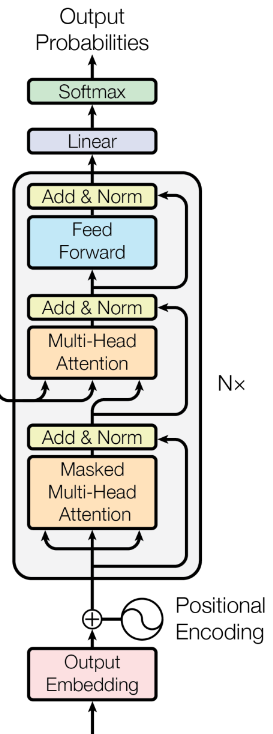
\includegraphics[width=3.5cm]{figures/fig1-q1-transformer-decoder.png}
    \caption{Transformer decoder}
    \label{fig:transformer-decoder}
\end{wrapfigure}

You will first implement a decoder-only transformer model. 
An outline of the code is provided for you in \texttt{model.py}. This outline contains all the 
class and function declarations that are expected for the submission.
\textbf{Do not modify the classes, functions, or their arguments. Do not import new Python dependencies. This may break the automatic code test pipeline and result in failed unit tests.}
You should aim to have an efficient implementation for the model to train in a reasonable amount of time. This means calling PyTorch functions whenever possible, and also means that you should not write matrix operations using a for loop.
That said, you may not use layers or functions (e.g., {\tt torch.nn.TransformerDecoder}) that make implementation trivial. If you are unsure whether using something is acceptable, ask course staff.
\newline


Recall the Transformer Decoder from Lecture 2, shown in Figure~\ref{fig:transformer-decoder}.
There are four classes within the transformer that you are expected to implement:
\begin{enumerate}
    \item \texttt{MultiHeadAttention} - the ``Masked Multi-head Attention'' module.
    \item \texttt{FeedForward} - the ``Feed Forward'' module.
    \item \texttt{DecoderBlock} - a single decoder block, as described in ``The Decoder Step-by-Step'' in Lecture 2. Note that since we are implementing the decoder only, you do not need to implement the Encoder-Decoder Multi-Head Attention or the second ``Add \& Norm'' operation. 
    \item \texttt{DecoderLM} - the full decoder model: the embedding step, multiple decoder blocks, and the final output logits.
\end{enumerate}

\noindent \textbf{[Question 1.1]} (\emph{Written, 5 points}): \href{https://aclanthology.org/E17-2025/}{Press and Wolf (2017)} propose a weight tying technique for projecting hidden states of a language model to token logits. Read this paper, and in a few sentences, explain what weight tying does.
\newline

\noindent Write your answer here:
\begin{tcolorbox}[fit,height=2cm, width=\linewidth, blank, borderline={1pt}{-2pt}]
% STUDENT SOLUTION HERE
\end{tcolorbox}

\noindent \textbf{[Question 1.2]} (\emph{Written, 5 points}): Let $d$ be the hidden size of the model, $v$ be the vocab size, $b$ be the batch size, and $s$ be the sequence length. Suppose you have hidden states $h \in \mathbb{R}^{b \times s \times d}$ and token embeddings $E \in \mathbb{R}^{v \times d}$ stored in PyTorch tensors. Write one line of Python code (potentially calling functions in PyTorch) that computes the token logits using weight tying.
\newline

\noindent
Write your answer here:
\begin{tcolorbox}[fit,height=2cm, width=\linewidth, blank, borderline={1pt}{-2pt}]
% STUDENT SOLUTION HERE
\end{tcolorbox}

\noindent \textbf{[Question 1.3]} (\emph{Coding, 25 points}): Complete \texttt{model.py}, implementing all of the classes above. All the unit tests are provided in the test script \texttt{test\_model.py}. Your implementation will be awarded points for each of the five unit tests that pass.
\newline

\section{Training the Transformer [85 points]}

Now that you have implemented the transformer, it is time to train the model! For ease of implementation and testing, we will provide the tokenized input for you. We will train on a subset of the C4 corpus\footnote{\url{https://huggingface.co/datasets/allenai/c4}}, which is itself a subset of the Common Crawl web corpus\footnote{\url{https://commoncrawl.org/}}. This dataset is downloaded automatically as a part of the training script, and there is no need for you to access it manually. \newline

An outline of the code is provided for you in \texttt{train.py}.
Keep in mind the various hyperparameters that are relevant for training: batch size, learning rate (and its scheduler), gradient accumulation, etc. These hyperparameters are read from a configuration file. We have provided sample configuration files for you for adjusting the hyperparameters.
There are five functions that you are expected to implement:
\begin{enumerate}
    \item \texttt{train} - the main training loop.
    \item \texttt{random\_batch\_sampler} - a data sampling function used in training that yields randomly shuffled batches of the data.
    \item \texttt{sequential\_batch\_sampler} - a data sampling function used in validation that yields a sequential pass through the data.
    \item \texttt{cosine\_lr\_schedule} - learning rate scheduler with Cosine annealing (see question 2.2).
    \item \texttt{compute\_language\_modeling\_loss} - the loss function used for training and evaluating the model.
\end{enumerate}

\noindent \textbf{[Question 2.1]} (\emph{Coding, 20 points}): Complete \texttt{train.py}, implementing the above functions.
All the unit tests are provided in the test script \texttt{test\_train.py}. Your implementation will be awarded points for each of the five unit tests that pass.
\newline

\noindent \textbf{[Question 2.2]} (\emph{Written, 10 points}): Cosine annealing with warmup is a commonly used dynamic learning rate strategy in training neural nets. It has two phases, in the warmup phase where $t \in [0,a)$, the learning rate increases linearly from 0 to $\mathrm{lr}_\text{max}$. In the annealing phase where $t \in [a,b)$, the learning rate decays from $\mathrm{lr}_\text{max}$ to $\mathrm{lr}_\text{min}$ following a half-cosine curve. When $t \ge b$, the learning rate stays at $\mathrm{lr}_\text{min}$. Figure~\ref{fig:cosine-schedule} shows an example of this schedule.

\begin{figure}[h!]
    \centering
    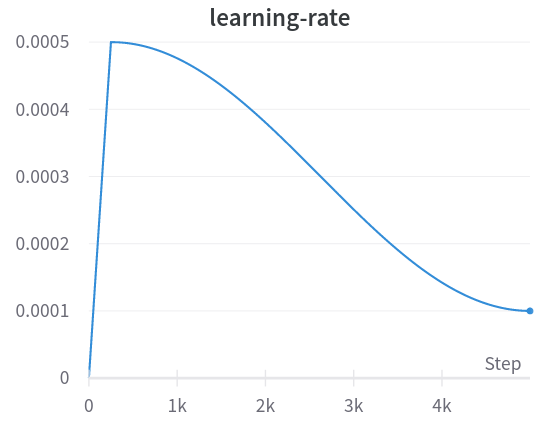
\includegraphics[width=0.5\linewidth]{figures/fig2-q2.2-cosine-schedule.png}
    \caption{Example Cosine Schedule}
    \label{fig:cosine-schedule}
\end{figure}

Using the symbols provided, write down two expressions, one for the learning rate during warmup and one for the learning rate during annealing.
\newline

\noindent
Write your expression for cosine annealing here:
\begin{tcolorbox}[fit,height=2cm, width=\linewidth, blank, borderline={1pt}{-2pt}]
% STUDENT SOLUTION HERE
\end{tcolorbox}

\noindent Why would one want to use cosine annealing? What are some advantages of cosine annealing over a constant learning rate? Write your answer here:
\begin{tcolorbox}[fit,height=2cm, width=\linewidth, blank, borderline={1pt}{-2pt}]
% STUDENT SOLUTION HERE
\end{tcolorbox}

\noindent \textbf{[Question 2.3]} (\emph{Written, 10 points}): What is the validation loss after training with the configuration provided in \texttt{GPT-tiny.yaml}? For approximately how many training steps should the model be trained to achieve optimal performance? Report the training loss curve (use a screenshot from weights \& biases: \url{https://wandb.ai/site}). 
\newline 

\noindent
Write the validation loss for \texttt{GPT-tiny} here:
\begin{tcolorbox}[fit,height=1cm, width=6cm, blank, borderline={1pt}{-2pt}]
% STUDENT SOLUTION HERE
\end{tcolorbox}

\noindent
Write the number of training steps needed for \texttt{GPT-tiny} here:
\begin{tcolorbox}[fit,height=1cm, width=6cm, blank, borderline={1pt}{-2pt}]
% STUDENT SOLUTION HERE
\end{tcolorbox}

\noindent
Include your training curve for \texttt{GPT-tiny} below:
\begin{tcolorbox}[fit,height=10cm, width=12cm, blank, borderline={1pt}{-2pt}]
% Replace the box with the figure below
\end{tcolorbox}

\clearpage
\begin{figure}[h!]
    \centering
    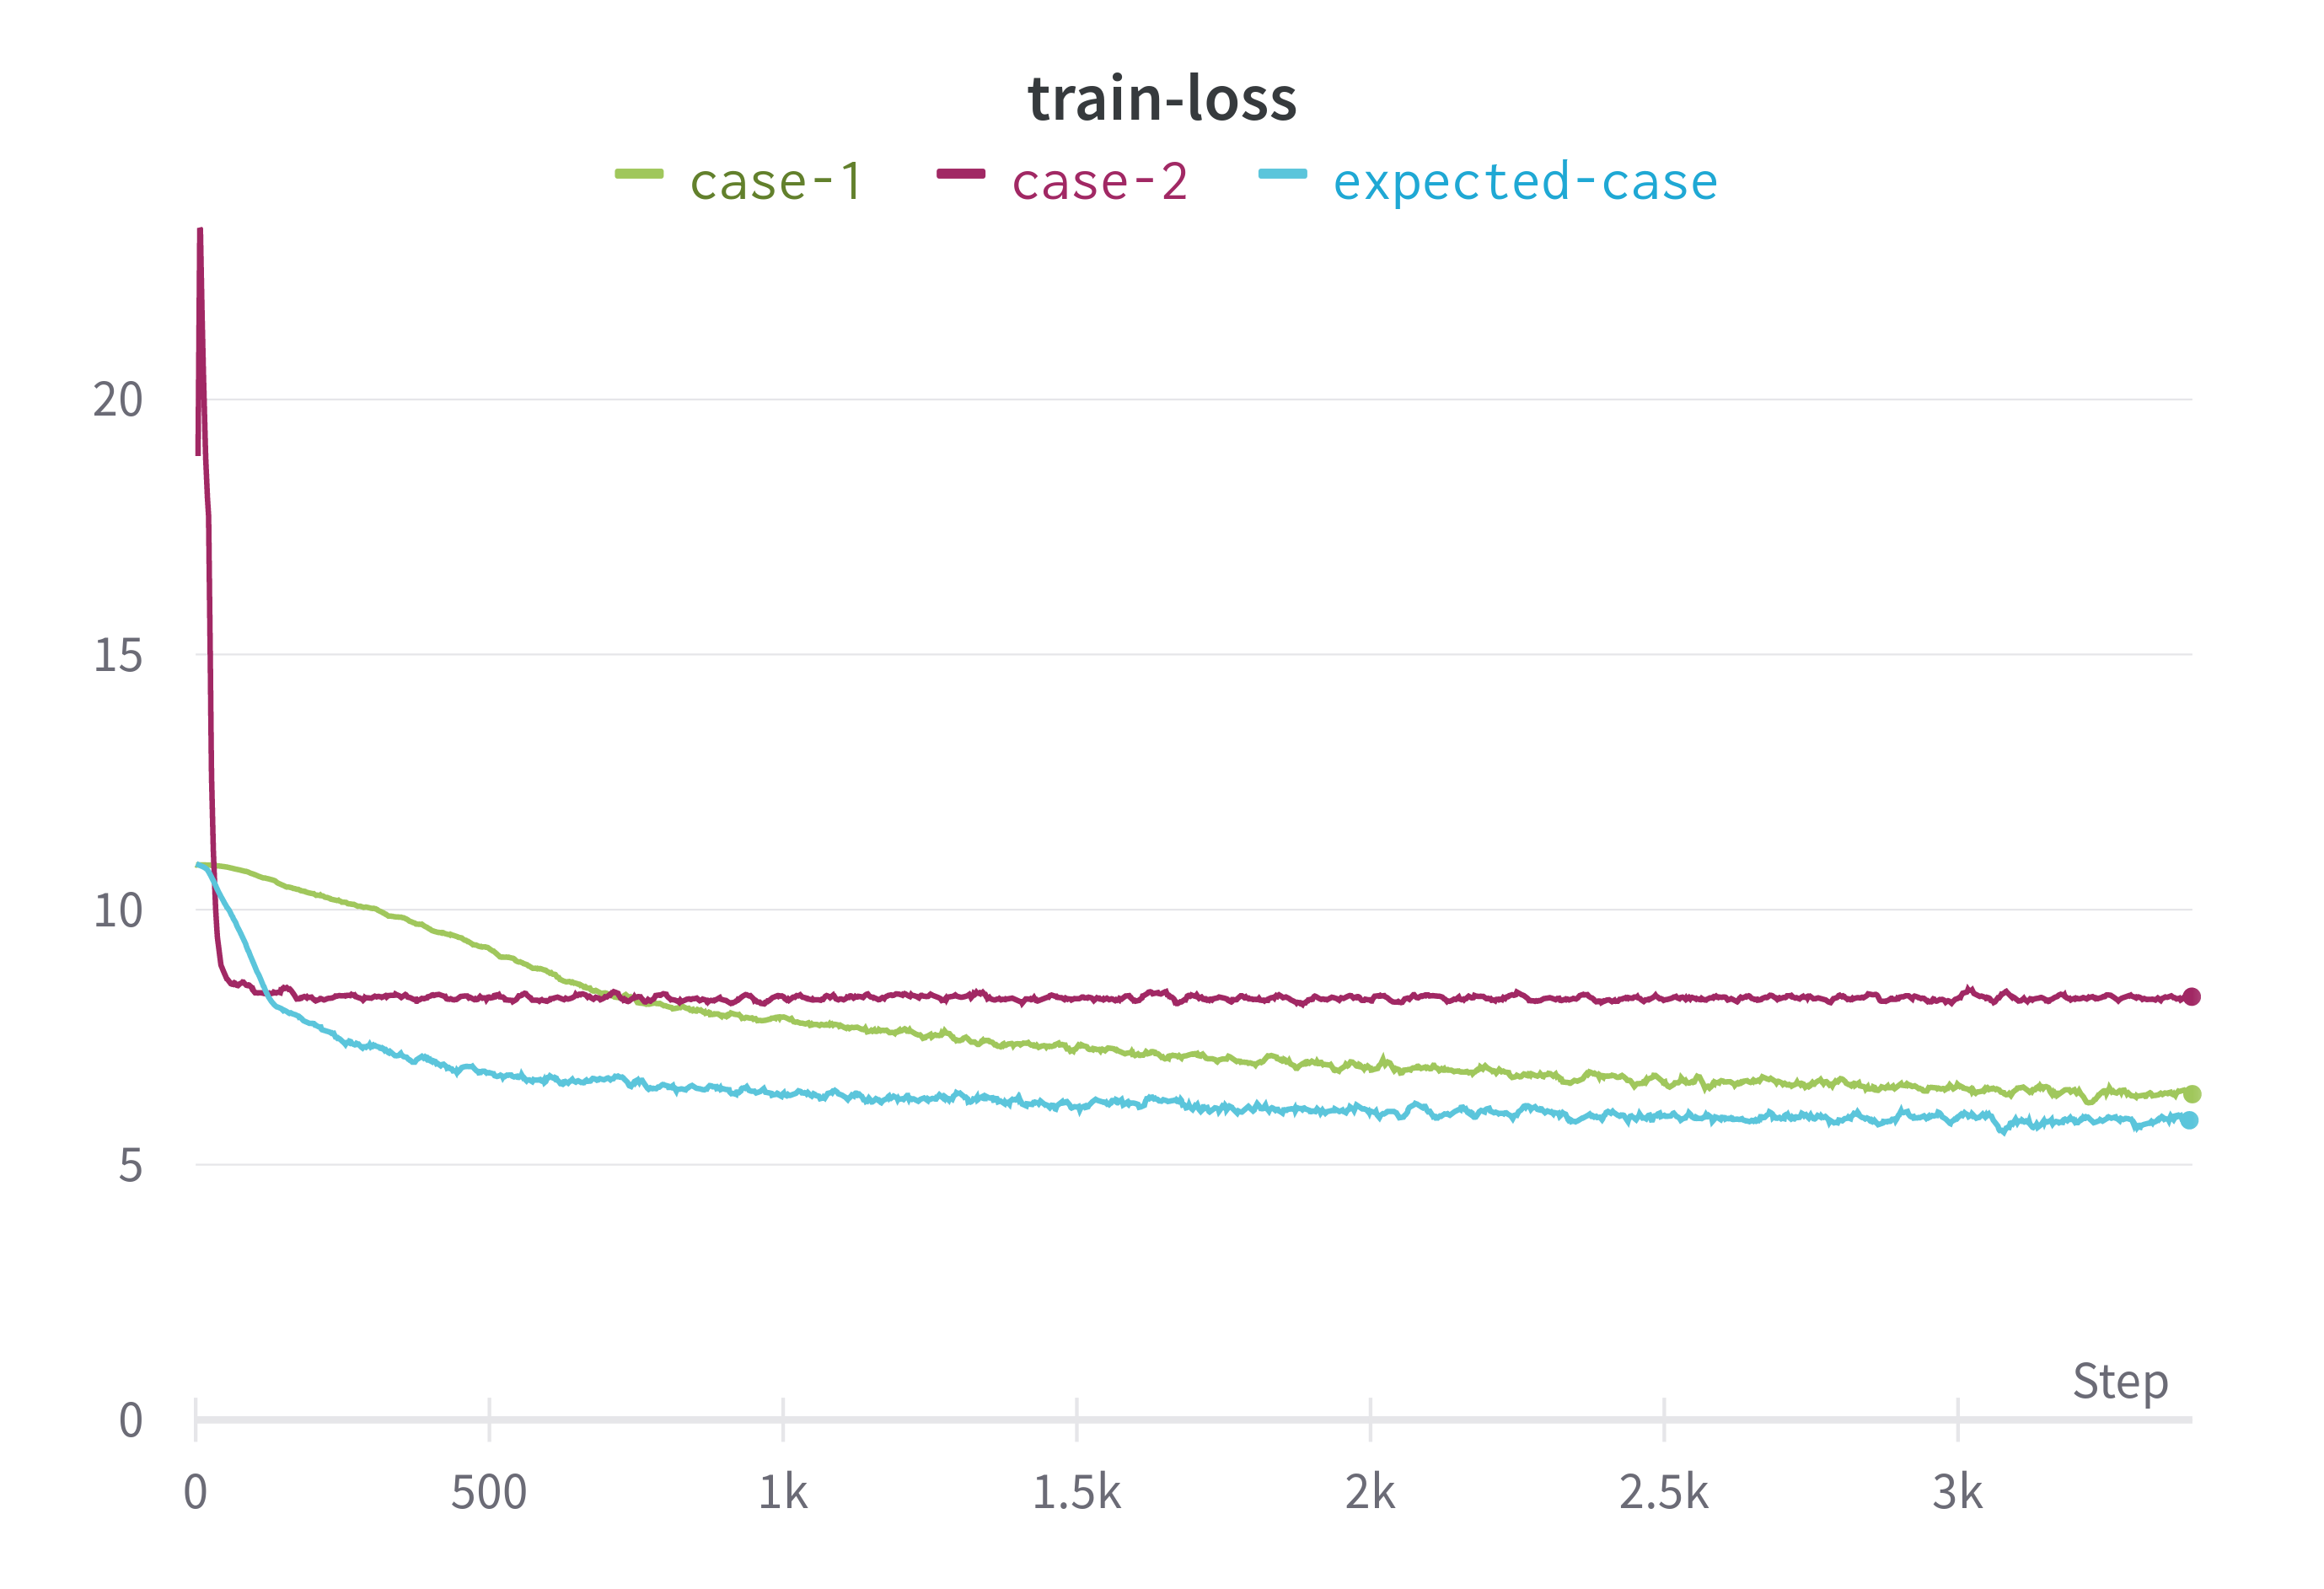
\includegraphics[width=0.75\linewidth]{figures/fig3-q2.4-broken-training.png}
    \caption{Broken training cases: case-1 and case-2}
    \label{fig:broken-training}
\end{figure}

\noindent \textbf{[Question 2.4]}: (\emph{Written, 5 points}) 
Figure~\ref{fig:broken-training} shows two mis-configured training runs, compared against their expected case with the proper configuration. For case-1 and case-2, in only a couple sentences each, can you explain what is wrong with the training setup? The loss function and transformer implementations are correct. \newline

\noindent
Write your answer here for case-1:
\begin{tcolorbox}[fit,height=2cm, width=\linewidth, blank, borderline={1pt}{-2pt}]
% STUDENT SOLUTION HERE
\end{tcolorbox}

\noindent
Write your answer here for case-2:
\begin{tcolorbox}[fit,height=2cm, width=\linewidth, blank, borderline={1pt}{-2pt}]
% STUDENT SOLUTION HERE
\end{tcolorbox}

\noindent \textbf{[Question 2.5]} (\emph{Written, 20 points}): Next, you will perform hyperparameter tuning. When optimizing neural networks, a common way to measure the total computation needed is with floating-point operations (FLOPs). E.g., a single multiply-add of floats is counted as a FLOP.
%
Assume that you have a compute budget of 1e+15 FLOPs for training. Experiment with your model and training hyperparameters to find the best configuration when training with at most 1e+15 FLOPs (the code for computing the number of FLOPs used to train a model is provided in \texttt{train.py}). Note that the FLOP limit is intentionally low: it should not take more than 10 minutes per hyperparameter test. \newline

As long as you stay within the FLOP budget, you are free to modify any of the following hyperparameters, all of which affect the number of FLOPs used: model hyperparameters such as \texttt{n\_embd}, \texttt{n\_head}, \texttt{n\_positions} and \texttt{n\_layer}; and training hyperparameters such as \texttt{batch\_size}, \texttt{seq\_len}, \texttt{grad\_accumulation\_steps}, and \texttt{num\_training\_steps}.
%
Describe your experiment: report results for \textbf{at most five} hyperparameter results: describe what hyperparameter values are modified, and their resulting validation perplexity (PPL). For your best performing setting, report the final configuration (YAML file) for this setting.
\newline

\noindent
Report your experiment procedure and results here:
\begin{tcolorbox}[fit,height=7cm, width=\linewidth, blank, borderline={1pt}{-2pt}]
% STUDENT SOLUTION HERE
\end{tcolorbox}

\noindent
Paste your final YAML configuration here:
\begin{tcolorbox}[fit,height=3cm, width=\linewidth, blank, borderline={1pt}{-2pt}]
% STUDENT SOLUTION HERE
\end{tcolorbox}

\noindent \textbf{[Question 2.6]} (\emph{Coding, 20 points}): Using the model configuration reported above, train your final model. For training your final model, you may train 100x more FLOPs (i.e. up to 1e+17 FLOPS), but do not change your model hyperparameters. Your final model should be able to achieve a PPL under 50 on the validation set.
Please include your final model checkpoint \texttt{model.pt} in your submission. We will verify your model with an offline correctness test, which will measure the perplexity on a test dataset (not provided). Submissions with PPL under 50 are guaranteed to get full score, and we will relax this requirement if needed.

\noindent
Report your final validation loss and PPL:
\begin{tcolorbox}[fit,height=1cm, width=6cm, blank, borderline={1pt}{-2pt}]
% STUDENT SOLUTION HERE
\end{tcolorbox}

\section{Using the Language Model for Downstream Tasks [40 points]}

\subsection*{Text Generation}

Next, you will use your trained LLM to generate text.
An outline of the code for text generation is provided for you in \texttt{generate.py}. To generate text, prompts must be provided to the LLM; we have provided an input file \texttt{prefixs.json} with sample inputs.
\newline

\noindent There are two functions that you are expected to implement:
\begin{enumerate}
    \item \texttt{generate} - given a \texttt{DecoderLM} and a list of prompts, generate tokens.
    \item \texttt{softmax\_with\_temperature} - convert a given a set of logits into probabilities with the softmax function, using temperature.
\end{enumerate}

\noindent \textbf{[Question 3.1]} (\emph{Coding, 10 points}): Complete \texttt{generate.py}, implementing the above functions. One unit test are provided in the test script \texttt{test\_generate.py}. Your implementation will be awarded points for passing the unit test and correctly implementing \texttt{generate}.
\newline

\noindent \textbf{[Question 3.2]} (\emph{Written, 5 points}):
Using the three prefixes provided in \texttt{prefixs.json}, report generations from the prompts. Repeat this process, experimenting with different temperature values and prompts. What happens to the generations if the temperature is near zero, or near one? Do you notice anything interesting with the generated text?
\newline

\noindent
Report your generations here:
\begin{tcolorbox}[fit,height=6cm, width=\linewidth, blank, borderline={1pt}{-2pt}]
% STUDENT SOLUTION HERE
\end{tcolorbox}
\clearpage

\noindent
Write your answer here:
\begin{tcolorbox}[fit,height=2cm, width=\linewidth, blank, borderline={1pt}{-2pt}]
% STUDENT SOLUTION HERE
\end{tcolorbox}

\noindent \textbf{[Question 3.3]} (\emph{Written, 5 points}):
Beyond adjusting hyperparameters for sampling, how can the quality of generation be improved? Provide at least two suggestions for how generation quality can be improved and reasons why you expected an improvement. 
\newline

\noindent
Write your answer here:
\begin{tcolorbox}[fit,height=4cm, width=\linewidth, blank, borderline={1pt}{-2pt}]
% STUDENT SOLUTION HERE
\end{tcolorbox}

\subsection*{Sentiment Analysis}

Finally, your trained LLM can be used to perform sentiment analysis. An outline of the code for sentiment analysis is provided for in \texttt{classify.py}. To evaluate sentiment analysis, use the Yelp polarity dataset: a labelled dataset of positive/negative Yelp reviews. During inference, you will place the text into a Yelp text template and determine if the token ``good'' or ``bad'' is more likely.

\noindent There are two functions that you are expected to implement:
\begin{enumerate}
    \item \texttt{score} - score the next token given a list of prefix strings.
    \item \texttt{classify\_binary\_sentiment} - given a \texttt{DecoderLM} and a set of input texts, predict if the input texts are "positive" reviews.
\end{enumerate}

\noindent \textbf{[Question 3.4]} (\emph{Coding, 10 points}): Complete \texttt{classify.py}, implementing the above functions. 
One unit test are provided in the test script \texttt{test\_classify.py}. Your implementation will be awarded points for passing the unit test and correctly implementing \texttt{score}.
\newline
\clearpage

\noindent \textbf{[Question 3.5]} (\emph{Written, 5 points}): Report the classification accuracy on the Yelp polarity dataset \emph{without} calibration. Is the performance higher than random (50\%) or majority class (53.1\%)? Explain why this is the case.

\noindent
Classification accuracy without calibration:
\begin{tcolorbox}[fit,height=1cm, width=4cm, blank, borderline={1pt}{-2pt}]
% STUDENT SOLUTION HERE
\end{tcolorbox}

\noindent
Write your answer here:
\begin{tcolorbox}[fit,height=2cm, width=\linewidth, blank, borderline={1pt}{-2pt}]
% STUDENT SOLUTION HERE
\end{tcolorbox}

\noindent \textbf{[Question 3.6]} (\emph{Written, 5 points}): When applying language models directly to classification, the model can often be miscalibrated. An example of a model biased to the positive label is shown in Figure~\ref{miscalibrated}.
Assuming there are roughly the same number of positive and negative examples in the dataset, how can you find a better decision boundary for a miscalibrated model than the default value (0.5) without access to labels or a separate development set?
In other words, your calibration strategy should depend exclusively on the predicted $\mathbf{p}(\text{Positive})$ for all test instances.

Under this new decision boundary you came up with, report the classification accuracy on the Yelp polarity dataset.
Other than training a bigger model or training for longer, what are some other potential ways to improve the classification performance? \newline

\begin{figure}[h!]
    \centering
    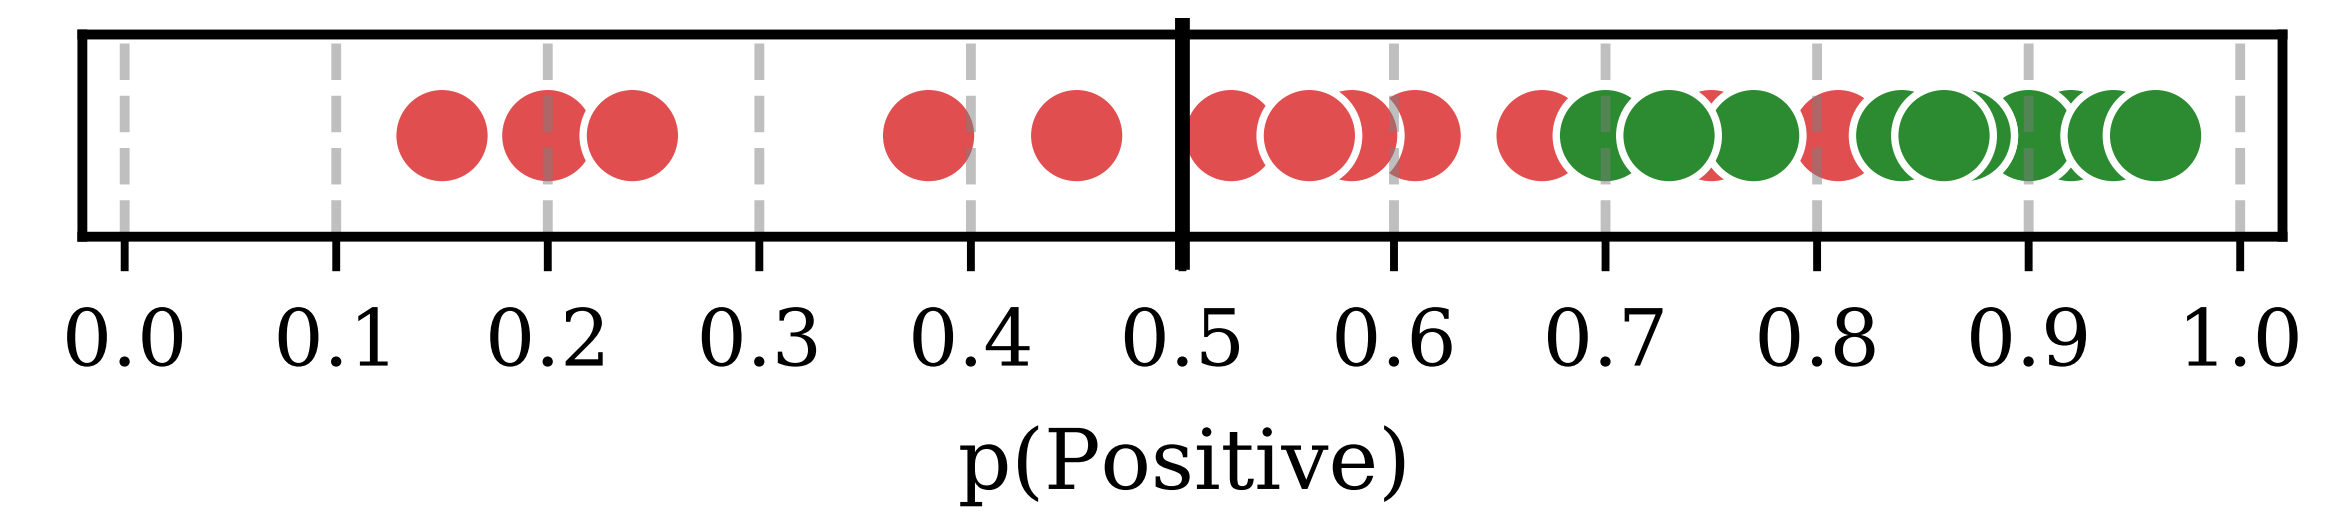
\includegraphics[width=0.75\linewidth]{figures/fig4-q3.6-calibration.png}
    \caption{A miscalibrated classifier that is biased to the positive class, taken from \href{https://arxiv.org/abs/2102.09690}{Zhao et al. (2021)}.
    Negative groundtruth examples are marked with \textcolor{mred}{$\newmoon$}, and positive groundtruth examples are marked with \textcolor{mgreen}{$\newmoon$}.
    Note: This figure is for illustration, and the plotted distribution will likely be different from the actual outputs of your model.}
    \label{miscalibrated}
\end{figure}

\noindent
Your proposed method of computing the calibrated decision boundary:
\begin{tcolorbox}[fit,height=2cm, width=\linewidth, blank, borderline={1pt}{-2pt}]
% STUDENT SOLUTION HERE
\end{tcolorbox}


\noindent
Classification accuracy with calibration:
\begin{tcolorbox}[fit,height=1cm, width=4cm, blank, borderline={1pt}{-2pt}]
% STUDENT SOLUTION HERE
\end{tcolorbox}

\noindent
Other ways to improve classification performance:
\begin{tcolorbox}[fit,height=2cm, width=\linewidth, blank, borderline={1pt}{-2pt}]
% STUDENT SOLUTION HERE
\end{tcolorbox}

\section{Optional: Give us Feedback}

Was this homework enjoyable? Was it too easy or too hard? Do you have any suggestions for making the homework run more smoothly? Giving us feedback is completely optional and will not factor into your grade. \newline

\noindent
Feedback:
\begin{tcolorbox}[fit,height=4cm, width=\linewidth, blank, borderline={1pt}{-2pt}]
% STUDENT SOLUTION HERE
\end{tcolorbox}

\end{document}
